\chapter{Analysis}

\section{Introduction}

\subsection{The Client and Users}
The client is the physics department of Long Road Sixth Form College, who have requested software to demonstrate the core concepts within the new specification AS Physics. The client has requested that the software can be used by both the students and the teachers both inside and outside of class, therefore, the software should work on college PCs without any additional resources (assuming the PC has Python3, OpenGL and PyQt installed, which is standard installation in Long Road Sixth Form). The simulation and rendering needs to work in real time (or faster) and it needs to be easy to use.

\subsection{The Current System}
The current system involves manually using physical equations with respect to \textit{t} (time), however, the current system does not show the progression between $t_0$ and $t_n$ it only shows the state at the beginning and at the end. The client feel that this doesn't show students actually how the objects move and interact with each other.

\subsubsection{Data Sources and Destinations}
	Because this system operates in a purely hypothetical context all of the inputs are user generated. The current system is always used to solve a problem or find a missing value in a formula, this missing value is nearly always positional and can always be calculated from given values, by a simple rearrangement of a formula. These rearrangements are generated based on a small set of known equations and formulae.
	So usually, as a first step in approaching a question or a problem which requires a solution, the user identifies the initial variables, in effect these are the input into the system.\\In the broadest possible sense, the following flow is represented.
\begin{figure}[H]
	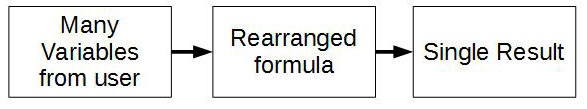
\includegraphics[width=\textwidth]{./Analysis/current_system_data_flow.JPG}
\end{figure}

\subsubsection{Algorithms}
	The process of identifying the variables and how they are to be used is relatively simple, the values that are to be used are given in the question and the output value is identified, then the the equation is rearranged OR an equation which has already been rearranged which uses all the input values to generate the output 
	


\section{Specific Requirements}
The specific requirements for this simulator can be derived from the Physics AS new specification (2015), a list of which are:
\begin{itemize}
	\item Gravity  - objects should be subject to gravity.
	\item Collisions
	\begin{itemize}
		\item Basic collisions - Objects should not overlap.
		\item Bounce - Objects should bounce (see momentum).
	\end{itemize}
	\item Kinematics - Objects should use the basic rules of kinematics to determine their movement.
	\item Forces - Objects should exert forces on each other, and react to forces and impulse.
	\item Centre of Gravity and Moment - Objects should have a centre of gravity, and they should have moments.
	\item Momentum and Impulse - Objects should simulate the effects of momentum and impulse according to Newton's laws.
\end{itemize}

The simulator program should also have the following utility features:
\begin{itemize}
	\item Save/Load Simulations - The program should be able to save and load simulations at a certain state.
	\item The ability to change the time scale of the simulation.
	\item The software needs to execute in approximately real time (at least 15fps).
	\item The software needs to be able to represent the physical objects as a set of binary objects in a database.

\end{itemize}

\section{Processing Requirements}
One of the key requirements for this system is that the simulation runs and renders smoothly, at approximately real time, this means that it is of paramount importance that the code is written in such a way that it executes quickly, and that it manages the host PC's resources efficiently. All of the college PCs have multi core processors, but they do not have dedicated GPUs which would ease the CPU strain for real-time physics simulation. This means that the system will have to use multi threading to accelerate the simulation and the rendering.

If all else fails, and the simulator doesn't render in real time, there should be an option to reduce the output resolution scaling, which should dramatically reduce the processing required to simulate and render.

\section{Data Flow}
\subsection{Input}
	The user will input some or all of the physical values into an input form. The simulation is designed to be open, so that the user can enter as many or as few properties as they want.

\subsection{Storage}
	The user's input will be stored in table within a database file. That data will then be used to generate an initial frame, which is then in turn stored in the same database. As each frame is generated, it'll store it in this same database file. This means that there are three 'frames' stored in the database: A pre-initial frame, which has the raw data that the user input, an initial frame which contains the generated data for the first frame; and the latest frame simulated. The following path will be followed: Render - Simulate - Store - Render - Simulate etc.

\subsection{Database}

\subsubsection{Entity Relationship Diagrams}
	Here is where I'll put the entity relationship diagrams

\subsubsection{Data flow diagrams}
%	DFDs I need to work out the dataflow diagrams of the original system.


\subsection{Output}
	The simulation data will be  converted into an updated series of shapes and positions which will be drawn to an OpenGL window. To the user, this should appear to be a stable, flowing animation of the shapes moving, rather than a set of individual frames.
	
\section{Measurable Goals}
	This project will be complete when the following conditions are met:
	\begin{itemize}
		\item All of the above objectives have been met
		\item The program executes with no unhandled errors.
%		\item Anything else?
	\end{itemize}
	I have allocated \textit{x} months from planning to handing the software to the client, this should provide ample time to complete these objectives.
	




\section{Summary}
In short, the system that I propose will add another degree of interactivity to the AS course, and it'll accurately demonstrate a comprehensive set of physical laws and relationships that will be covered in the new specification AS. The software will be a freely script-able physics engine, rather than a fixed set of customisable simulations - it could maybe even be developed into a 2d game engine, this means that the user will be able to create a 2D world from scratch and use it to demonstrate, experiment, or just play with any physical object that they can define.
